Jako další byl vytvořen zjednodušený případ užití celého systému podle stanovanených požadavků, především s ohledem na zvolený systém anonymizace hlasovacích lístků, tak jak byl popsán v kapitole \ref{section:blindSign}.


\begin{figure}[h]
	\centering
	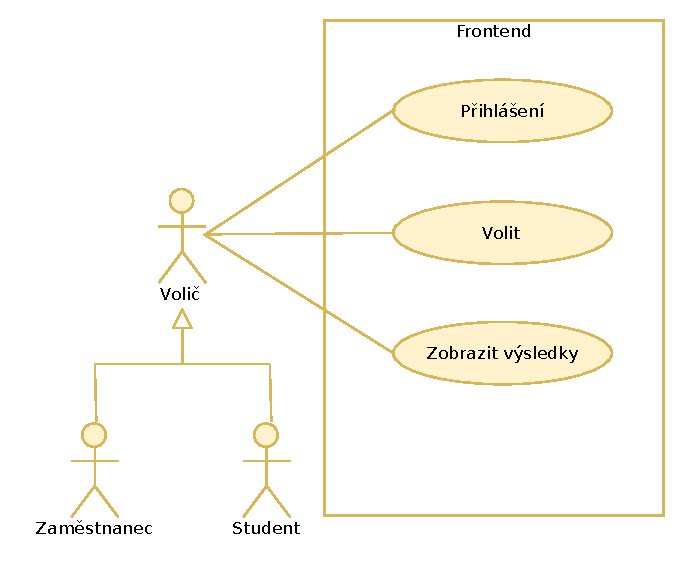
\includegraphics[width=0.5\linewidth]{svg/useCaseVolic.eps}
	\captionsetup{width=0.5\linewidth}
	\caption[Případ užití systému Frontend]{Případ užití systému Frontend (zdroj: vlastní)}
\end{figure}
\begin{figure}[h]
	\centering
	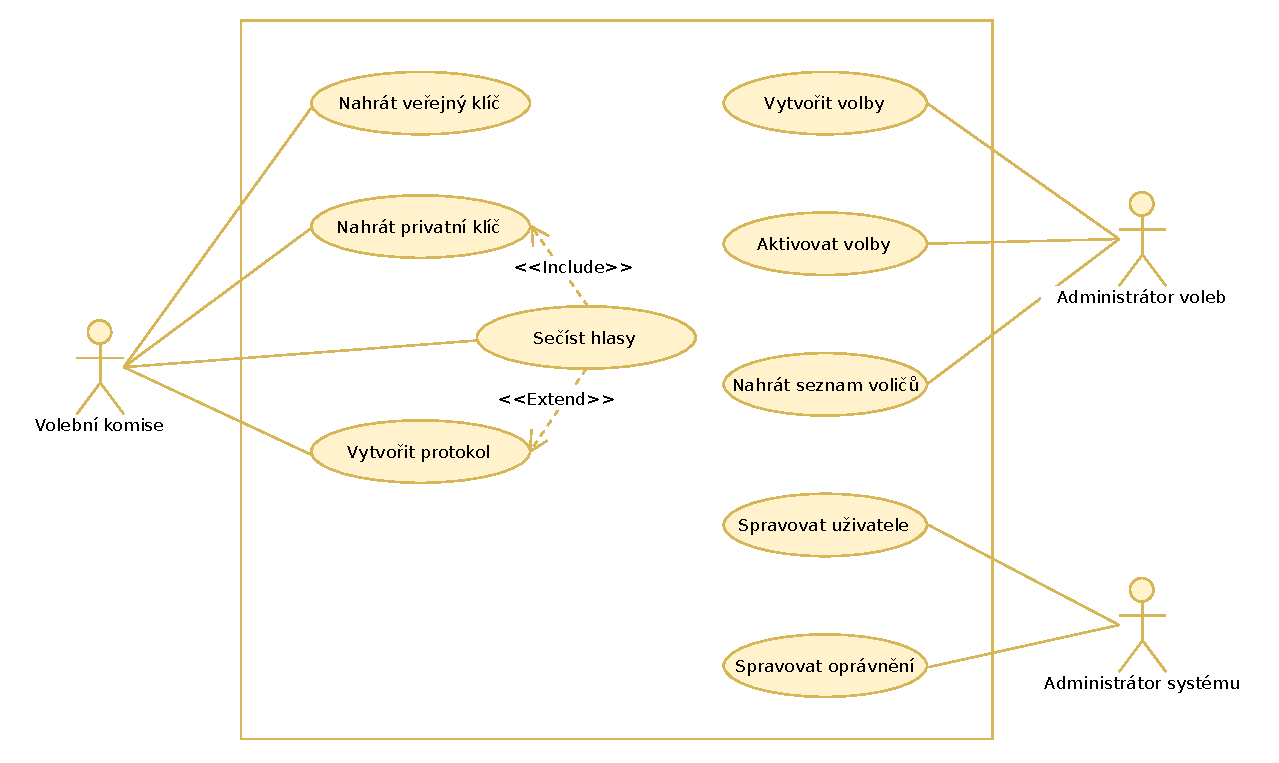
\includegraphics[width=\linewidth]{svg/useCaseBackend.eps}
	\captionsetup{width=\linewidth}
	\caption[Případ užití systému Backend]{Případ užití systému Backend (zdroj: vlastní)}
\end{figure}